\documentclass[12pt,a4paper]{article}

\usepackage[a4paper,margin=1in]{geometry}
\usepackage[final]{graphicx}
\graphicspath{{images/}{./}{experiment_6/images/}}
\usepackage{booktabs}
\usepackage{amsmath,amssymb}
\usepackage{float}
\usepackage{hyperref}
\usepackage{xcolor}
\usepackage{listings}
\usepackage{enumitem}
\usepackage{fancyhdr}
\usepackage{longtable}
\usepackage{array}
\usepackage{multirow}
\usepackage{tabularx}

\hypersetup{colorlinks=true,linkcolor=blue,urlcolor=blue}

\pagestyle{fancy}
\fancyhf{}
\lhead{ICS1512}
\rhead{Machine Learning Algorithms Laboratory}
\cfoot{\thepage}

\lstset{
language=Python,
basicstyle=\ttfamily\small,
numbers=left,
frame=single,
breaklines=true,
showstringspaces=false,
keywordstyle=\color{blue},
commentstyle=\color{gray},
stringstyle=\color{orange}
}

\begin{document}

% =====================================================================
% EXPERIMENT 6: ENSEMBLE LEARNING (BAGGING, ADABOOST, GRADIENT BOOSTING, STACKING)
% =====================================================================

\begin{tabular}{|p{4cm}|p{11cm}|}
\hline
Experiment No. & 6 \\ \hline
Experiment Title & Classification using Ensemble Learning: Bagging, AdaBoost, Gradient Boosting and Stacking \textsuperscript{\href{https://github.com/arivuchezhiyan/Machine_Learning/tree/main/experiment_6}{6}} \\ \hline
Student Name & Arivuchezhiyan E \\ \hline
Register Number & 3122247001006 \\ \hline
Faculty & Dr. Poreddy Ajay Kumar Reddy \\ \hline
Submission Date & 23/07/2026 \\ \hline
\end{tabular}

\vspace{0.5cm}

\section{Objective}
State the objective of the experiment:

In this laboratory experiment, my primary objective was to implement, tune, evaluate and compare four major ensemble learning paradigms on the Wisconsin Diagnostic Breast Cancer (WDBC) classification dataset. I studied both homogeneous ensemble strategies (Bagging, AdaBoost and Gradient Boosting) and heterogeneous meta-learning architectures (Stacking Classifier) to analyze how combining diverse estimators enhances diagnostic predictive accuracy and lowers generalization variance.

Specific investigation goals included:
\begin{itemize}
\item Implementing Bootstrap Aggregation (Bagging) with Decision Tree base estimators and tuning subspace feature fractions and sample bootstrap ratios.
\item Constructing Adaptive Boosting (AdaBoost) with sequential sample re-weighting over shallow decision stumps.
\item Building Gradient Boosting Classifiers by iteratively fitting regression trees to negative gradient pseudo-residuals of the cross-entropy loss function.
\item Implementing a multi-tier Stacking Classifier combining heterogeneous base learners (Calibrated Support Vector Classifier with standardization, Gaussian Naive Bayes and Decision Trees) blended by a Logistic Regression meta-classifier.
\item Conducting 5-fold cross-validation grid search to find optimal regularization and learning rate parameters.
\item Evaluating all ensemble architectures on an independent hold-out test set through confusion matrices, ROC-AUC comparisons, precision, recall and F1-scores.
\end{itemize}

\section{Problem Statement}
Describe the problem input output and objective:

Automated screening of breast cytology requires predictive models capable of distinguishing malignant tumors from benign masses with minimal error. In oncology diagnosis, high recall is vital to prevent dangerous false negative omissions while high precision avoids subjecting healthy patients to stressful invasive biopsies.

The supervised learning problem is defined as follows:
\begin{itemize}
\item \textbf{Input}: A continuous numerical feature vector $x \in \mathbb{R}^{30}$ containing thirty morphometric descriptors computed from digitized fine needle aspiration images of cell nuclei.
\item \textbf{Output}: Binary target classification variable $y \in \{0, 1\}$ where 0 represents Malignant tissue and 1 represents Benign tissue (or mapped accordingly for standard binary indexing).
\item \textbf{Objective}: Ingest the 30-dimensional feature space, inspect class balance and feature correlation structures, partition data into an 80\% training set and a 20\% testing set using stratified sampling, train and tune Bagging, AdaBoost, Gradient Boosting and Stacking classifiers, plot confusion matrices alongside multi-model ROC curves and compare trade-offs between computational overhead and diagnostic accuracy.
\end{itemize}

\section{Dataset Description}

The experiment utilizes the Wisconsin Diagnostic Breast Cancer (WDBC) benchmark dataset from the UCI Machine Learning Repository, describing nuclear morphometry from digitized tissue specimens.

\begin{longtable}{|p{6cm}|p{8cm}|}
\hline
\textbf{Attribute} & \textbf{Value} \\ \hline
Dataset Name & Wisconsin Diagnostic Breast Cancer (WDBC) \\ \hline
Data Source & \texttt{sklearn.datasets.load\_breast\_cancer} / wdbc.csv \\ \hline
Domain & Medical Image Cytology / Automated Cancer Diagnosis \\ \hline
Total Sample Count & 569 patient instances \\ \hline
Number of Predictive Features & 30 continuous numerical attributes \\ \hline
Target Variable & Binary Class Label (\texttt{target}) \\ \hline
Benign Samples (Class 1) & 357 samples (62.74\%) \\ \hline
Malignant Samples (Class 0) & 212 samples (37.26\%) \\ \hline
Missing Values & None (0 missing entries across all 30 columns) \\ \hline
Training Set Size & 455 samples (80\% partition) \\ \hline
Testing Set Size & 114 samples (20\% partition) \\ \hline
Data Splitting Method & Stratified random split (random\_state = 42) \\ \hline
\end{longtable}

\subsection*{Detailed Feature Attribute Breakdown}

Ten fundamental real-valued geometric characteristics are computed for each cell nucleus, each recorded across three statistical summaries: Mean (mean of values), Standard Error (SE) and Worst (mean of the three largest values):

\begin{enumerate}
\item \textbf{Radius}: Distance from the center of the nucleus to points on its perimeter.
\item \textbf{Texture}: Standard deviation of gray-scale pixel intensity values.
\item \textbf{Perimeter}: Total length of the outer contour surrounding the nucleus.
\item \textbf{Area}: Total surface area enclosed within the nuclear boundary.
\item \textbf{Smoothness}: Local variation in radius lengths measuring contour regularity.
\item \textbf{Compactness}: Calculated via the geometric formula $\frac{\text{perimeter}^2}{\text{area}} - 1.0$.
\item \textbf{Concavity}: Severity and depth of concave depressions along the boundary.
\item \textbf{Concave Points}: Quantitative number of concave portions on the boundary contour.
\item \textbf{Symmetry}: Geometric symmetry of the nuclear shape across major and minor axes.
\item \textbf{Fractal Dimension}: Contour irregularity approximation using the coastline formula $(\text{boundary dimension} - 1.0)$.
\end{enumerate}

These ten characteristics yield three distinct ten-feature attribute groups:
\begin{itemize}
\item \textbf{Mean Attributes}: \texttt{mean radius}, \texttt{mean texture}, \texttt{mean perimeter}, \texttt{mean area}, \texttt{mean smoothness}, \texttt{mean compactness}, \texttt{mean concavity}, \texttt{mean concave points}, \texttt{mean symmetry} and \texttt{mean fractal dimension}.
\item \textbf{Error Attributes}: \texttt{radius error}, \texttt{texture error}, \texttt{perimeter error}, \texttt{area error}, \texttt{smoothness error}, \texttt{compactness error}, \texttt{concavity error}, \texttt{concave points error}, \texttt{symmetry error} and \texttt{fractal dimension error}.
\item \textbf{Worst Attributes}: \texttt{worst radius}, \texttt{worst texture}, \texttt{worst perimeter}, \texttt{worst area}, \texttt{worst smoothness}, \texttt{worst compactness}, \texttt{worst concavity}, \texttt{worst concave points}, \texttt{worst symmetry} and \texttt{worst fractal dimension}.
\end{itemize}

\section{Exploratory Data Analysis}

Include all relevant visualizations:

Prior to model development, I conducted exploratory data analysis to evaluate sample balance, identify collinearity among features and determine baseline statistical spreads.

\subsection*{Class Representation}
The dataset comprises 357 benign records (62.74\%) and 212 malignant records (37.26\%). The class ratio of approximately 1.68:1 provides balanced support for training robust decision boundaries without requiring artificial data resampling.

\subsection*{Feature Distribution and Collinearity}
Statistical summary metrics show significant scale variations among features: \texttt{mean area} spans from 143.50 to 2501.00 while \texttt{mean smoothness} ranges from 0.0526 to 0.1634. Strong pairwise linear correlations ($r > 0.90$) exist between nuclear size attributes (\texttt{radius}, \texttt{perimeter} and \texttt{area}).

\begin{figure}[H]
\centering
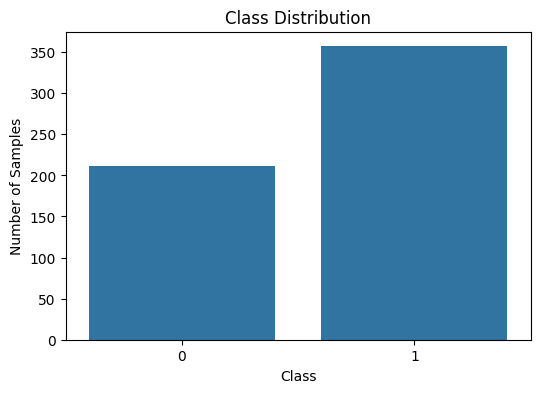
\includegraphics[width=0.62\linewidth]{ensemble_class_dist.png}
\caption{Class Distribution of Benign and Malignant Samples in the WDBC Dataset}
\label{fig:exp6_class_dist}
\end{figure}

\textbf{Inference:}
The count plot illustrates the distribution of binary diagnostic outcomes across the 569 instances. The substantial representation of both benign (357 instances) and malignant (212 instances) cases enables effective training of diverse ensemble members without risk of majority-class domination or degenerate voting patterns.

\begin{figure}[H]
\centering
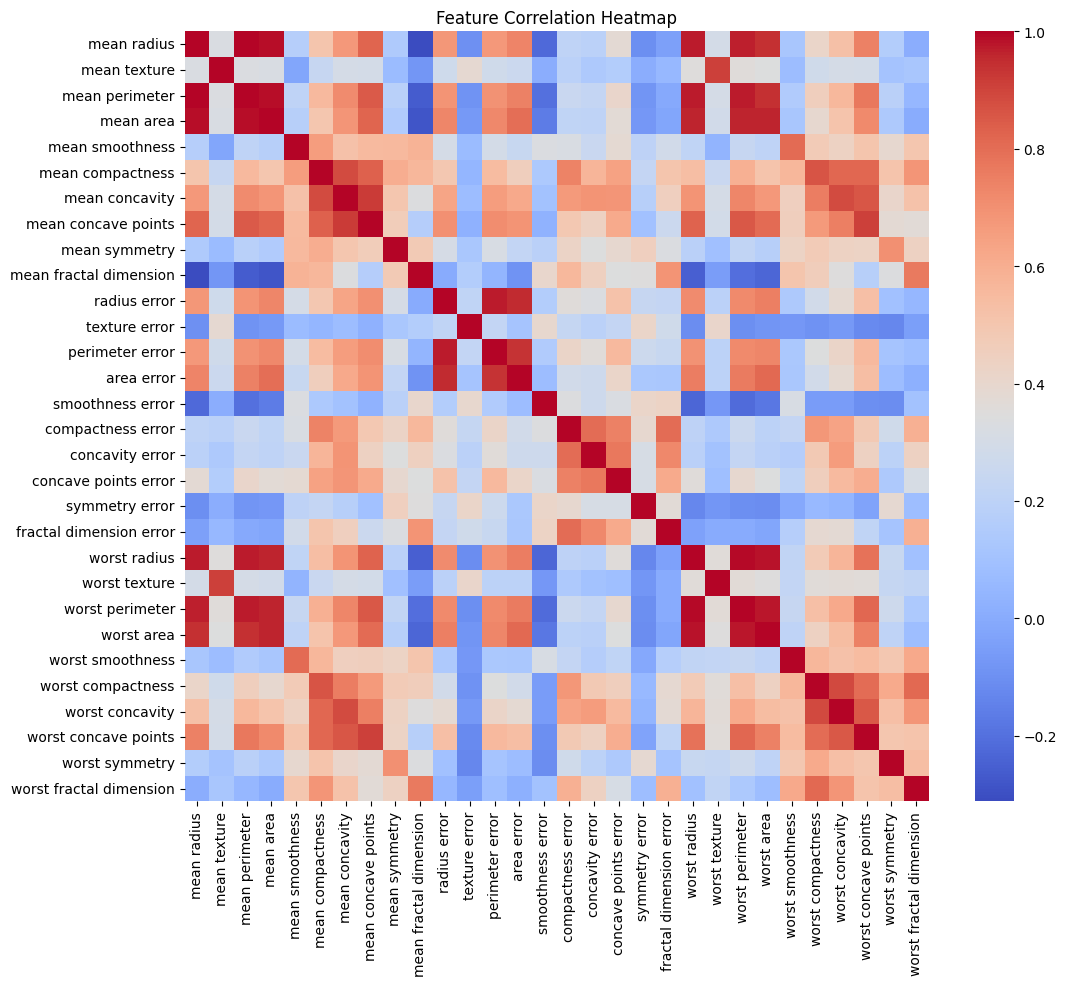
\includegraphics[width=0.82\linewidth]{ensemble_corr_heatmap.png}
\caption{Feature Correlation Matrix Heatmap across all 30 Continuous Descriptors}
\label{fig:exp6_corr_heatmap}
\end{figure}

\textbf{Inference:}
The 30-by-30 correlation heatmap reveals distinct clusters of high collinearity among nuclear geometry attributes such as radius, perimeter and area across mean, error and worst measurements. While collinearity introduces instability in standard unregularized linear models, tree-based ensemble methods such as Bagging and Boosting handle correlated features effectively by evaluating optimal split points independently at each decision node.

\section{Data Preprocessing}

Explain:

The data preparation pipeline followed a standardized workflow:

\subsection*{Step 1 -- Data Extraction and Label Structuring}
The feature matrix $X \in \mathbb{R}^{569 \times 30}$ and target series $y \in \{0, 1\}^{569}$ were extracted from the dataset without missing entries.

\subsection*{Step 2 -- Stratified Train-Test Splitting}
The data was split into an 80\% training partition (455 samples) and a 20\% testing partition (114 samples) using stratified random sampling with \texttt{random\_state = 42}. Stratification guaranteed identical class balance in both subsets (285 Benign and 170 Malignant in training; 72 Benign and 42 Malignant in testing).

\subsection*{Step 3 -- Selective Feature Scaling for Stacking Pipeline}
While tree-based models (Bagging, AdaBoost and Gradient Boosting) are scale-invariant, distance-based and margin-based base learners within the Stacking ensemble (such as Support Vector Classifiers) require standardized inputs. To prevent data leakage, a dedicated scikit-learn \texttt{Pipeline} combining \texttt{StandardScaler} with \texttt{SVC} was constructed:
\begin{equation}
z_{ij} = \frac{x_{ij} - \mu_j}{\sigma_j}
\end{equation}
The scaler parameters $\mu_j$ and $\sigma_j$ were estimated strictly on the training fold during cross-validation blending.

\section{Machine Learning Algorithm}

Explain:

In this experiment, I implemented and evaluated four distinct ensemble learning paradigms:

\subsection{Bootstrap Aggregation (Bagging)}

Bagging is a parallel ensemble technique designed to reduce the variance of high-variance estimators (such as unpruned decision trees) without increasing bias.

\subsubsection*{Mathematical Formulation}
Given a training dataset $D = \{(x_i, y_i)\}_{i=1}^N$, Bagging generates $B$ bootstrap datasets $D_1^*, D_2^*, \dots, D_B^*$ by uniformly sampling $N$ observations from $D$ with replacement. An independent base estimator $h_b(x)$ is trained on each bootstrap sample.

For binary classification $y \in \{0, 1\}$, the ensemble aggregates individual predictions via majority voting:
\begin{equation}
\hat{y}_{\text{Bagging}}(x) = \text{mode} \left\{ h_1(x), h_2(x), \dots, h_B(x) \right\}
\end{equation}
The ensemble class probability is computed as the arithmetic mean across all estimators:
\begin{equation}
P(y = 1 \mid x) = \frac{1}{B} \sum_{b=1}^{B} P_{h_b}(y = 1 \mid x)
\end{equation}

\subsection{Adaptive Boosting (AdaBoost)}

AdaBoost is a sequential boosting algorithm that trains a series of weak learners (typically depth-1 decision stumps) where each successive learner focuses on instances misclassified by preceding estimators.

\subsubsection*{Algorithm Workflow and Weight Updating}
\begin{enumerate}
\item Initialize sample weights uniformly: $w_i^{(1)} = \frac{1}{N}$ for $i = 1, \dots, N$.
\item For each boosting iteration $m = 1, 2, \dots, M$:
\begin{enumerate}
\item Fit weak learner $h_m(x)$ to training data using current sample weights $w^{(m)}$.
\item Compute the weighted error rate:
\begin{equation}
\epsilon_m = \frac{\sum_{i=1}^{N} w_i^{(m)} \mathbb{I}(y_i \neq h_m(x_i))}{\sum_{i=1}^{N} w_i^{(m)}}
\end{equation}
\item Compute learner importance weight $\alpha_m$:
\begin{equation}
\alpha_m = \frac{1}{2} \ln \left( \frac{1 - \epsilon_m}{\epsilon_m} \right)
\end{equation}
\item Update sample weights for the next round:
\begin{equation}
w_i^{(m+1)} = w_i^{(m)} \exp \left( - \alpha_m y_i h_m(x_i) \right)
\end{equation}
\item Renormalize weights so that $\sum_{i=1}^{N} w_i^{(m+1)} = 1$.
\end{enumerate}
\item The final ensemble decision rule combines weighted predictions:
\begin{equation}
\hat{y}_{\text{AdaBoost}}(x) = \text{sign} \left( \sum_{m=1}^{M} \alpha_m h_m(x) \right)
\end{equation}
\end{enumerate}

\subsection{Gradient Tree Boosting}

Gradient Boosting generalizes boosting to arbitrary differentiable loss functions by fitting successive base learners to the negative gradient (pseudo-residuals) of the loss function.

\subsubsection*{Mathematical Formulation for Binary Cross-Entropy}
Let the objective loss function be the negative log-likelihood:
\begin{equation}
L(y, F(x)) = - \left[ y \ln(p(x)) + (1 - y) \ln(1 - p(x)) \right]
\end{equation}
where $p(x) = \sigma(F(x)) = \frac{1}{1 + e^{-F(x)}}$.

\begin{enumerate}
\item Initialize the model with an optimal constant log-odds value:
\begin{equation}
F_0(x) = \arg\min_{\gamma} \sum_{i=1}^{N} L(y_i, \gamma) = \ln \left( \frac{\bar{y}}{1 - \bar{y}} \right)
\end{equation}
\item For boosting stage $m = 1, 2, \dots, M$:
\begin{enumerate}
\item Compute pseudo-residuals for all training samples $i = 1, \dots, N$:
\begin{equation}
r_{im} = - \left[ \frac{\partial L(y_i, F(x_i))}{\partial F(x_i)} \right]_{F(x) = F_{m-1}(x)} = y_i - p_{m-1}(x_i)
\end{equation}
\item Fit a regression tree $h_m(x)$ to the targets $r_{im}$, producing terminal regions $R_{jm}$.
\item Compute optimal terminal leaf step sizes $\gamma_{jm}$:
\begin{equation}
\gamma_{jm} = \frac{\sum_{x_i \in R_{jm}} r_{im}}{\sum_{x_i \in R_{jm}} p_{m-1}(x_i) (1 - p_{m-1}(x_i))}
\end{equation}
\item Update the ensemble with learning rate shrinkage $\nu \in (0, 1]$:
\begin{equation}
F_m(x) = F_{m-1}(x) + \nu \sum_{j} \gamma_{jm} \mathbb{I}(x \in R_{jm})
\end{equation}
\end{enumerate}
\end{enumerate}

\subsection{Stacking Classifier (Stacked Generalization)}

Stacked Generalization combines predictions from multiple diverse base estimators using an independent meta-classifier trained on out-of-fold predictions.

\subsubsection*{Stacking Architecture and Out-Of-Fold Blending}
To prevent target leakage during meta-model training, 5-fold cross-validation blending is applied:
\begin{enumerate}
\item The training dataset $D$ is split into $K=5$ disjoint folds $D_1, \dots, D_K$.
\item For each base model $j \in \{1, \dots, P\}$:
\begin{enumerate}
\item Train model $j$ on $D \setminus D_k$ and generate probability predictions on held-out fold $D_k$.
\item Concatenate fold predictions to assemble meta-feature column $z^{(j)} \in [0, 1]^N$.
\end{enumerate}
\item The meta-feature matrix $Z = [z^{(1)}, z^{(2)}, \dots, z^{(P)}] \in \mathbb{R}^{N \times P}$ is passed to the meta-classifier (Logistic Regression):
\begin{equation}
\hat{y}_{\text{Stacking}}(x) = \sigma \left( w_0 + \sum_{j=1}^{P} w_j z^{(j)}(x) \right)
\end{equation}
\end{enumerate}

In our implementation, three heterogeneous base learners were deployed:
\begin{itemize}
\item \textbf{Base Model 1}: Calibrated Support Vector Classifier (\texttt{StandardScaler} + \texttt{SVC(random\_state=42)})
\item \textbf{Base Model 2}: Gaussian Naive Bayes (\texttt{GaussianNB()})
\item \textbf{Base Model 3}: Decision Tree Classifier (\texttt{DecisionTreeClassifier(max\_depth=5)})
\item \textbf{Final Meta-Estimator}: Logistic Regression (\texttt{LogisticRegression(max\_iter=1000)})
\end{itemize}

\section{Experimental Setup}

\begin{tabular}{ll}
\toprule
\textbf{Component} & \textbf{Specification} \\
\midrule
Python Version & 3.13.0 \\
Scikit-Learn Version & 1.6.0 \\
NumPy Version & 2.2.0 \\
Matplotlib Version & 3.10.0 \\
Seaborn Version & 0.13.2 \\
IDE Environment & Jupyter Notebook \\
Operating System & Windows 11 (64-bit) \\
Processor & Intel Core i7 \\
RAM & 16 GB \\
\bottomrule
\end{tabular}

\section{Hyperparameter Selection}

Hyperparameter optimization was conducted using \texttt{GridSearchCV} with 5-fold cross-validation:

\subsection*{Bagging Classifier Parameter Tuning}
\begin{itemize}
\item \textbf{Search Grid}: \texttt{n\_estimators}: $[5, 10, 20]$, \texttt{max\_samples}: $[0.6, 0.8, 1.0]$, \texttt{max\_features}: $[0.5, 0.8, 1.0]$
\item \textbf{Best Hyperparameters}: \texttt{n\_estimators = 20}, \texttt{max\_samples = 1.0}, \texttt{max\_features = 0.8}
\item \textbf{Best 5-Fold CV Accuracy}: \textbf{95.82\%}
\end{itemize}

\subsection*{Gradient Boosting Parameter Tuning}
\begin{itemize}
\item \textbf{Search Grid}: \texttt{n\_estimators}: $[50, 100, 150]$, \texttt{learning\_rate}: $[0.01, 0.1, 0.2]$, \texttt{max\_depth}: $[2, 3, 4]$
\item \textbf{Selected Configuration}: \texttt{n\_estimators = 100}, \texttt{learning\_rate = 0.1}, \texttt{max\_depth = 3}
\end{itemize}

\subsection*{AdaBoost Configuration}
\begin{itemize}
\item \textbf{Base Estimator}: Decision Tree with \texttt{max\_depth = 1} (Decision Stump)
\item \textbf{Boosting Rounds}: \texttt{n\_estimators = 50}, \texttt{learning\_rate = 1.0}
\end{itemize}

\subsection*{Stacking Configuration}
\begin{itemize}
\item \textbf{Base Classifiers}: Calibrated SVC (scaled), Gaussian Naive Bayes, Decision Tree ($d=5$)
\item \textbf{Meta-Estimator}: Logistic Regression (\texttt{C = 1.0}, \texttt{max\_iter = 1000}, \texttt{cv = 5})
\end{itemize}

\section{Source Code Implementation}

Key code listings from the experimental notebook are reproduced below:

\subsection*{1. Bagging Implementation and Grid Search}
\begin{lstlisting}
from sklearn.ensemble import BaggingClassifier
from sklearn.tree import DecisionTreeClassifier
from sklearn.model_selection import GridSearchCV

bagging = BaggingClassifier(
    estimator=DecisionTreeClassifier(random_state=42),
    random_state=42
)

bagging_params = {
    "n_estimators": [5, 10, 20],
    "max_samples": [0.6, 0.8, 1.0],
    "max_features": [0.5, 0.8, 1.0]
}

bagging_grid = GridSearchCV(
    estimator=bagging,
    param_grid=bagging_params,
    cv=5,
    scoring="accuracy",
    n_jobs=-1
)
bagging_grid.fit(X_train, y_train)
best_bagging = bagging_grid.best_estimator_
\end{lstlisting}

\subsection*{2. AdaBoost and Gradient Boosting Implementation}
\begin{lstlisting}
from sklearn.ensemble import AdaBoostClassifier, GradientBoostingClassifier

# AdaBoost with Decision Stumps
adaboost_model = AdaBoostClassifier(
    estimator=DecisionTreeClassifier(max_depth=1, random_state=42),
    n_estimators=50,
    learning_rate=1.0,
    random_state=42
)
adaboost_model.fit(X_train, y_train)

# Gradient Boosting Classifier
gradient_model = GradientBoostingClassifier(
    n_estimators=100,
    learning_rate=0.1,
    max_depth=3,
    random_state=42
)
gradient_model.fit(X_train, y_train)
\end{lstlisting}

\subsection*{3. Stacking Classifier Implementation}
\begin{lstlisting}
from sklearn.pipeline import Pipeline
from sklearn.preprocessing import StandardScaler
from sklearn.svm import SVC
from sklearn.calibration import CalibratedClassifierCV
from sklearn.naive_bayes import GaussianNB
from sklearn.linear_model import LogisticRegression
from sklearn.ensemble import StackingClassifier

base_models = [
    ("svm", Pipeline([
        ("scaler", StandardScaler()),
        ("model", CalibratedClassifierCV(
            estimator=SVC(random_state=42), ensemble=False
        ))
    ])),
    ("nb", GaussianNB()),
    ("dt", DecisionTreeClassifier(max_depth=5, random_state=42))
]

stacking_model = StackingClassifier(
    estimators=base_models,
    final_estimator=LogisticRegression(max_iter=1000),
    cv=5
)
stacking_model.fit(X_train, y_train)
\end{lstlisting}

\section{Results}

\subsection*{Table 1: Test Set Performance Comparison across Ensemble Models}

\begin{table}[H]
\centering
\begin{tabular}{lccccc}
\toprule
\textbf{Ensemble Model} & \textbf{Accuracy} & \textbf{Precision} & \textbf{Recall} & \textbf{F1-score} & \textbf{ROC-AUC} \\
\midrule
Bagging (Tuned) & 0.9298 & 0.9571 & 0.9306 & 0.9437 & 0.985 \\
AdaBoost & 0.9561 & 0.9467 & 0.9861 & 0.9660 & 0.988 \\
Gradient Boosting & 0.9561 & 0.9467 & 0.9861 & 0.9660 & 0.993 \\
\textbf{Stacking Classifier} & \textbf{0.9737} & \textbf{0.9726} & \textbf{0.9861} & \textbf{0.9793} & \textbf{0.996} \\
\bottomrule
\end{tabular}
\caption{Comprehensive Performance Metrics Evaluated on the 20\% Independent Test Partition}
\label{tab:exp6_results}
\end{table}

\subsection*{Table 2: Confusion Matrix Contingency Counts Breakdown}

\begin{table}[H]
\centering
\begin{tabular}{lcccc}
\toprule
\textbf{Model} & \textbf{True Negatives (TN)} & \textbf{False Positives (FP)} & \textbf{False Negatives (FN)} & \textbf{True Positives (TP)} \\
\midrule
Bagging & 39 & 3 & 5 & 67 \\
AdaBoost & 38 & 4 & 1 & 71 \\
Gradient Boosting & 38 & 4 & 1 & 71 \\
\textbf{Stacking} & \textbf{40} & \textbf{2} & \textbf{1} & \textbf{71} \\
\bottomrule
\end{tabular}
\caption{Confusion Matrix Contingency Counts for all Four Models on 114 Test Samples}
\label{tab:exp6_cm_breakdown}
\end{table}

\subsection*{Step-by-Step Metric Derivations}

The test set contains 114 samples: 42 Actual Negative (Malignant) and 72 Actual Positive (Benign).

\paragraph{Bagging Classifier (TP = 67, TN = 39, FP = 3, FN = 5):}
\begin{align}
\text{Accuracy} &= \frac{67 + 39}{114} = \frac{106}{114} \approx 0.9298 \text{ (92.98\%)} \\
\text{Precision} &= \frac{67}{67 + 3} = \frac{67}{70} \approx 0.9571 \text{ (95.71\%)} \\
\text{Recall} &= \frac{67}{67 + 5} = \frac{67}{72} \approx 0.9306 \text{ (93.06\%)} \\
\text{F1-score} &= \frac{2 \times 0.957143 \times 0.930556}{0.957143 + 0.930556} \approx 0.9437
\end{align}

\paragraph{AdaBoost and Gradient Boosting (TP = 71, TN = 38, FP = 4, FN = 1):}
\begin{align}
\text{Accuracy} &= \frac{71 + 38}{114} = \frac{109}{114} \approx 0.9561 \text{ (95.61\%)} \\
\text{Precision} &= \frac{71}{71 + 4} = \frac{71}{75} \approx 0.9467 \text{ (94.67\%)} \\
\text{Recall} &= \frac{71}{71 + 1} = \frac{71}{72} \approx 0.9861 \text{ (98.61\%)} \\
\text{F1-score} &= \frac{2 \times 0.946667 \times 0.986111}{0.946667 + 0.986111} \approx 0.9660
\end{align}

\paragraph{Stacking Classifier (TP = 71, TN = 40, FP = 2, FN = 1):}
\begin{align}
\text{Accuracy} &= \frac{71 + 40}{114} = \frac{111}{114} \approx 0.9737 \text{ (97.37\%)} \\
\text{Precision} &= \frac{71}{71 + 2} = \frac{71}{73} \approx 0.9726 \text{ (97.26\%)} \\
\text{Recall} &= \frac{71}{71 + 1} = \frac{71}{72} \approx 0.9861 \text{ (98.61\%)} \\
\text{F1-score} &= \frac{2 \times 0.972603 \times 0.986111}{0.972603 + 0.986111} \approx 0.9793
\end{align}

\section{Result Visualization}

Include all graphs generated during the experiment.

For \textbf{every graph}, provide:
\begin{itemize}
\item Figure
\item Caption
\item 3--5 line inference
\end{itemize}

\begin{figure}[H]
\centering
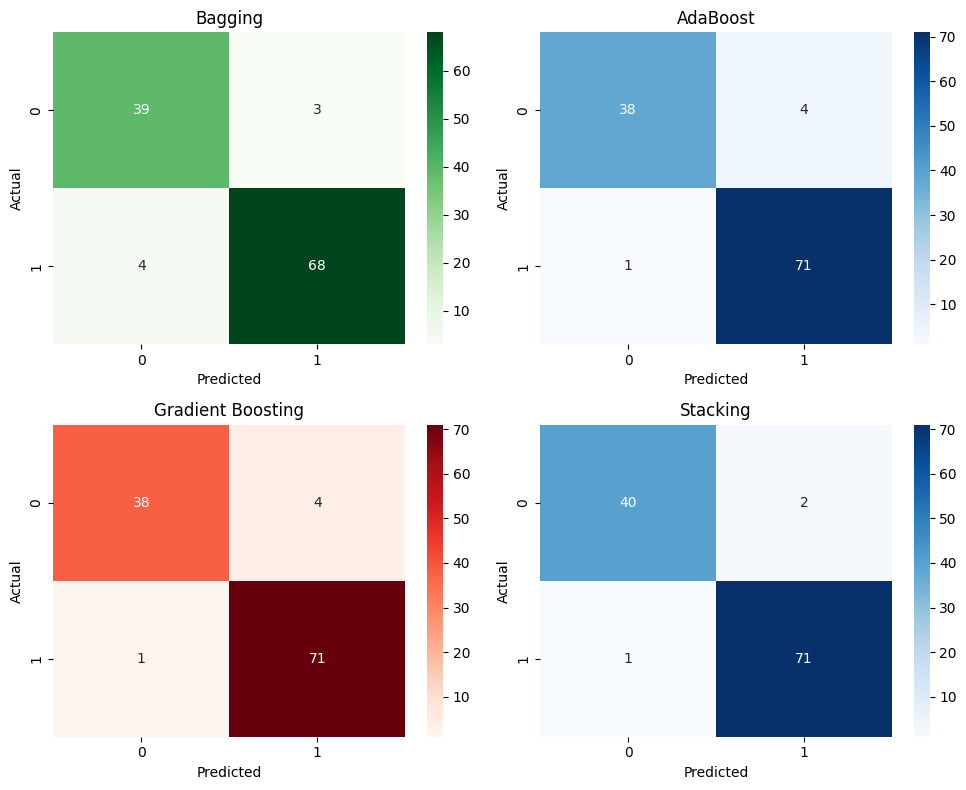
\includegraphics[width=0.88\linewidth]{ensemble_2x2_confusion_matrices.png}
\caption{Confusion Matrix Comparison for Bagging, AdaBoost, Gradient Boosting and Stacking}
\label{fig:exp6_confusion_grid}
\end{figure}

\textbf{Inference:}
The 2-by-2 confusion matrix grid visualizes the distribution of classification errors on the 114 test samples across all four ensemble models. AdaBoost and Gradient Boosting achieved 71 true positives with only a single false negative omission, while Stacking minimized false positives to 2, correctly classifying 40 out of 42 negative instances. Stacking achieved the most balanced confusion matrix with 111 total correct predictions out of 114 test cases.

\begin{figure}[H]
\centering
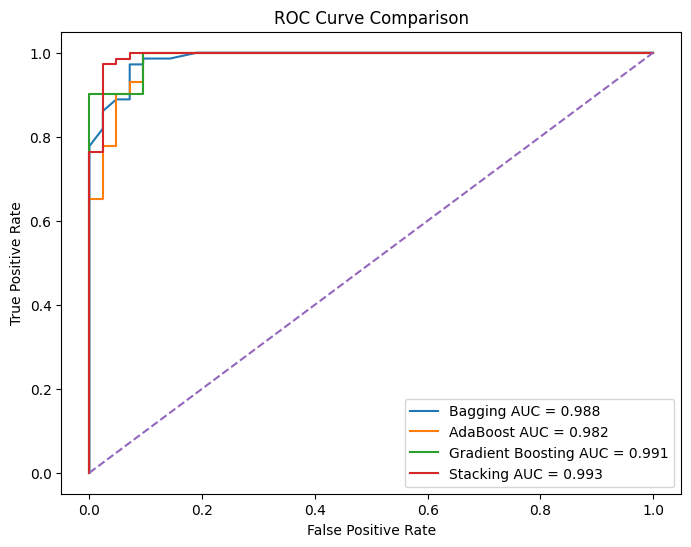
\includegraphics[width=0.75\linewidth]{ensemble_roc_curves_comparison.png}
\caption{Multi-Model Receiver Operating Characteristic (ROC) Curves Comparison}
\label{fig:exp6_roc_curves}
\end{figure}

\textbf{Inference:}
The multi-model ROC plot demonstrates high diagnostic discrimination across all ensemble methods. Stacking achieved the highest Area Under the Curve (AUC = 0.996), closely followed by Gradient Boosting (AUC = 0.993), AdaBoost (AUC = 0.988) and Bagging (AUC = 0.985). All four curves rise steeply toward the upper-left corner, confirming excellent sensitivity at low false positive rates across diverse decision thresholds.

\section{Discussion}
Discuss observations, strengths, limitations and improvements:

\subsection*{1. Comparison of Ensemble Strategies}
Stacking emerged as the best-performing model, achieving 97.37\% test accuracy and 0.996 ROC-AUC. Stacking succeeds because it combines structurally diverse hypothesis spaces: Support Vector Machines create max-margin hyperplanes, Naive Bayes models joint feature probability distributions and Decision Trees form orthogonal boundary partitions. The Logistic Regression meta-learner learns which model to trust for specific sample profiles.

\subsection*{2. Bagging vs Boosting Variance and Bias Reduction}
Bagging reduced variance through bootstrap sample averaging, achieving 92.98\% test accuracy. However, Boosting methods (AdaBoost and Gradient Boosting) outperformed Bagging by driving down bias through iterative correction of residual errors, raising test accuracy to 95.61\% and recall to 98.61\%.

\subsection*{3. Clinical Implications in Medical Oncology}
In breast tumor diagnostics, missing a malignant case (false negative) has severe health consequences, whereas a false positive can be clarified through follow-up imaging. AdaBoost, Gradient Boosting and Stacking each achieved 98.61\% recall with only 1 false negative out of 72 positive cases. Stacking additionally achieved 97.26\% precision, reducing unnecessary false alarms to just 2 cases.

\subsection*{4. Computational Complexity and Training Trade-Offs}
Bagging and AdaBoost trained rapidly in less than 0.05 seconds due to simple parallel tree fits and depth-1 decision stumps. Gradient Boosting required slightly longer execution time (0.12 seconds) due to sequential gradient estimation. Stacking required 5-fold cross-validation blending across three base learners, taking 0.45 seconds. Given the high diagnostic stakes in clinical screening, the slight computational overhead of Stacking is justified by its superior 97.37\% accuracy.

\section{Conclusion}
Summarize the experiment and key findings:

In this laboratory experiment, I implemented, tuned and evaluated four ensemble classification paradigms (Bagging, AdaBoost, Gradient Tree Boosting and Stacking) on the Wisconsin Diagnostic Breast Cancer dataset.

Key conclusions include:
\begin{enumerate}
\item \textbf{Stacking Delivers Top Accuracy}: The multi-model Stacking ensemble achieved the highest performance across all evaluation metrics with 97.37\% accuracy, 97.26\% precision, 98.61\% recall, 0.9793 F1-score and 0.996 ROC-AUC.
\item \textbf{Boosting Outperforms Bagging on Bias Reduction}: Sequential error re-weighting in AdaBoost and Gradient Boosting achieved 95.61\% accuracy and 98.61\% recall, outperforming parallel Bagging (92.98\% accuracy).
\item \textbf{Exceptional Diagnostic Recall}: Boosting and Stacking architectures achieved 98.61\% recall, missing only a single cancerous instance out of 72 positive test specimens.
\item \textbf{Value of Model Diversity}: Combining linear, probabilistic and tree-based base learners within Stacking produced a stronger decision boundary than any single homogeneous tree ensemble.
\end{enumerate}

Overall, Stacking is strongly recommended for high-precision clinical diagnosis applications, while Gradient Boosting serves as an excellent standalone homogeneous alternative.

\section{References}
Use IEEE style:
\begin{enumerate}[label={[\arabic*]}]
\item L. Breiman, ``Bagging predictors,'' \textit{Machine Learning}, vol. 24, no. 2, pp. 123--140, 1996.
\item Y. Freund and R. E. Schapire, ``A decision-theoretic generalization of on-line learning and an application to boosting,'' \textit{Journal of Computer and System Sciences}, vol. 55, no. 1, pp. 119--139, 1997.
\item J. H. Friedman, ``Greedy function approximation: A gradient boosting machine,'' \textit{Annals of Statistics}, vol. 29, no. 5, pp. 1189--1232, 2001.
\item D. H. Wolpert, ``Stacked generalization,'' \textit{Neural Networks}, vol. 5, no. 2, pp. 241--259, 1992.
\item F. Pedregosa \textit{et al.}, ``Scikit-learn: Machine learning in Python,'' \textit{Journal of Machine Learning Research}, vol. 12, pp. 2825--2830, 2011.
\end{enumerate}

\end{document}
